\section{MPEG Immersive Video Standard}\label{sec:TMIV}

In this section, we briefly introduce the workflow and components of MIV codec~\cite{tmiv_doc,BDDF+21}.

\begin{figure}[tbh]
    \centering
    \subfigure[]{
        \label{fig:TMIV_encode}
        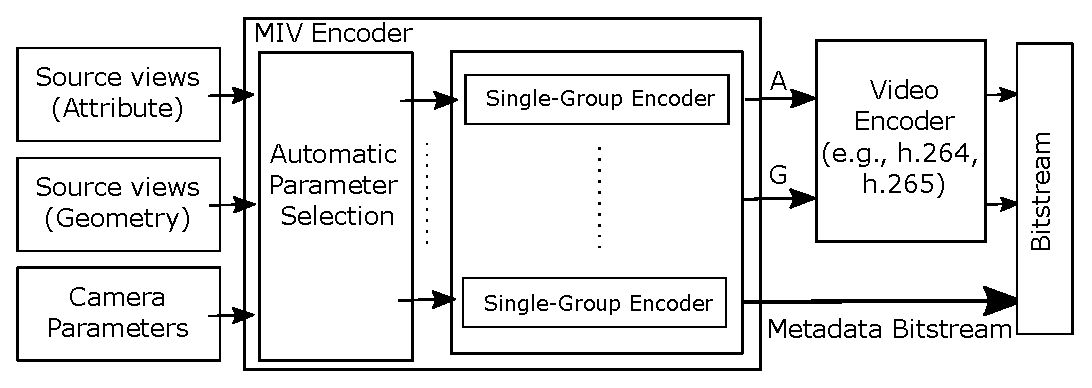
\includegraphics[width=.48\textwidth]{figs/TMIV_encode.eps}
    }
    \\
    \subfigure[]{
        \label{fig:TMIV_decode}
        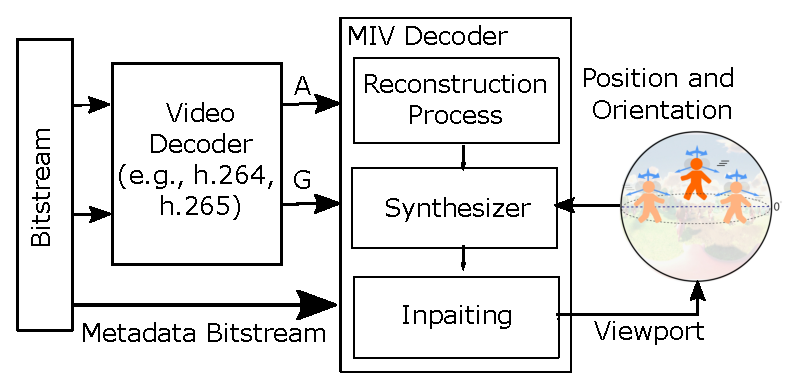
\includegraphics[width=.42\textwidth]{figs/TMIV_decode.eps}
    }
    \caption{The high-level overview of process flow of TMIV: (a) Encoder and (b) Decoder.}
    \label{fig:TMIV_codec}
\end{figure}

Fig.~\ref{fig:TMIV_encode} shows the high-level workflow of MIV encoder. The inputs of MIV encoder are {\em source views}. Each source view is composed of attribute (texture) videos, geometric (depth) videos, and camera parameters. MIV encoder do the following process to compress source views:
\begin{itemize}
    \item {\bf Automatic parameter selection.} MIV encoder automatically calculate the parameters for compression, e.g., assessing geometric video quality, splitting source views into multiple group according to configuration, and labeling source views in each group.
    \item {\bf Single-group encoders.} MIV encoder encodes each group of source views separately. In each group, 
    the encoder chooses several views as the basic view according to the label of source view, and remove the duplicate area in other source views. The basic view and remaining area of other views are packed into rectangle video frames, which are called {\em atlases}. Fig.~\ref{fig:atlas_example} show the example of atlases. 
\end{itemize}

\begin{figure}
    \centering
    \includegraphics[width=.38\textwidth]{figs/atlas_example.png}
    \caption{The example of atlases. The left picture is attribute atlas, and the right picture is geometric altas.}
    \label{fig:atlas_example}
\end{figure}

The outputs of MIV encoder are attribute atlases, geometric atlases, and metadata bitstream. The atlases are further compressed by video codec, and multiplexed with metadata bitstream as a single bitstream.

Fig.~\ref{fig:TMIV_decode} shows the high-level workflow of MIV decoder. The inputs pf MIV decoder is the bitstream contains atlases bitstream, and metadata bitstream. The video decoder first be employed to decompress attribute atlases and geometric atlases. After that MIV decoder do the following process to decompress altases and synthesize the user's viewport.
\begin{itemize}
    \item {\bf Reconstruction process.} The MIV decoder reconstruct the source view by using the data in atlases.
    \item {\bf Synthesizer.} The MIV decoder employ view synthesis techniques to synthesize the user's viewport according to user's position and orientation. Specifically, the synthesizer warp the pixel of each source view to user's viewport according to depth information, and blending the pixel values from each source views.
    \item {\bf Inpainting.}  After synthesis, the synthesized result may contain holes without information. The inpainting process uses the information from neighbor pixels to calculate pixel value for holes.
\end{itemize}
The outputs of MIV decoder are user's viewport synthesized according to user's position and orientation.
